\section{Related Work}


\subsection{Efficient LLMs}

Efficient large language models have gained significant attention in recent research community, especially with the growing prominence of ChatGPT.
% Numerous strategies have been proposed to reduce the inference and fine-tuning costs of LLMs, with the majority of work concentrating on model quantization, model compression, instruct tuning, and delta tuning. However, these methods primarily focus on model parameters and do not take into account the input prompts during the generation process.
Most of these methods aim to reduce the costs of inference and fine-tuning by modifying the model parameters through quantization~\cite{dettmers2022gptint, frantar2023optq, xiao2022smoothquant}, compression~\cite{frantar2023sparsegpt}, instruct tuning~\cite{alpaca,vicuna2023,xu2023wizardlm}, or delta tuning~\cite{hu2022lora}. %However, they overlook the role of input prompts during the generation process.

% In addition to the aforementioned works, 
A line of studies attempt to optimize inference costs from the perspective of the input prompts.
% by focusing on the prompt perspective.
Motivated by the observation of the abundance of identical text spans between the input and the generated result, \citet{yang2023inference} directly copy tokens from prompts for decoding to accelerate the inference process of LLMs.
% Specifically, with the observation that there is a partial overlap between the input and the generated results, 
% \citet{yang2023inference} proposes a prompt copy method to accelerate the inference process of LLMs.
Some approaches focus on compressing prompts, specifically, learning special tokens via prompt tuning of LLMs to reduce the number of tokens to be processed during inference \cite{mu2023learning,ge2022extensible,wingate-etal-2022-prompt,chevalier2023adapting, ge2023context}. 
% Some works employ prompt tuning to fine-tune LLMs, learning unique tokens that represent specific tasks~\cite{mu2023learning}, prompts~\cite{wingate-etal-2022-prompt, chevalier2023adapting}, or style customization~\cite{ge2022extensible}, thus reducing the number of tokens that need to be processed during inference.
Unfortunately, these methods are usually tailored to particular tasks and some of them \cite{mu2023learning,chevalier2023adapting} even require to fine-tune the whole language model, which severely limits their application scenarios.
Furthermore, there are some studies~\cite{Chase_LangChain_2022,zhang2023mlcopilot} that attempt to utilize LLMs to summarize dialog or data, thereby forming memory and knowledge. However, these approaches require multiple invocations of LLMs, which are quite costly.

% In addition to the aforementioned methods, 
Some methods reduce the prompt length by selecting a subset of demonstrations.
For example, \citet{zhou2023efficient} introduces a reinforcement learning based algorithm to allocate a specific number of demonstrations for each question.
Some other methods focus on token pruning~\cite{goyal2020power,kim2021length,kim2022learned,rao2021dynamicvit,modarressi2022adapler} and token merging~\cite{bolya2023token}.
However, these approaches are proposed for smaller models such as BERT, ViT.
Moreover, they depend on fine-tuning the models or obtaining intermediate results during inference.
% \citet{zhou2023efficient} introduces a reinforcement learning (RL) based algorithm that allocates a specific number of demonstrations for each question, thereby reducing prompt length.

The most similar work to this paper is Selective-Context~\cite{li2023unlocking}, 
% Recently, \citet{li2023unlocking} proposes \textit{Selective-Context},
which evaluates the informativeness of lexical units by computing self-information with a small language model, and drops the less informative content for prompt compression. 
% a prompt compression algorithm based on self-information phrase granularity, 
% Selective-Context that employs self-information to filter out less informative content
This paper is inspired by Selective-Context and further proposes a coarse-to-fine framework to address its limitations. 
% However, this method ignores the conditional relationships between compressed contents and lays aside the alignment of the target LLM and the small base language model.
% In this paper, we introduce a token-level iterative prompt compression method to better model the conditional dependencies between compressed tokens, and propose an instruction tuning based method to narrow the aforementioned distribution gap.
% We further propose a budget controller and perform demonstration-level compression to  maintain semantic integrity under high compression ratios.

% \textcolor{blue}{In this paper, Ours v.s. Selective-Context ... This paragraph may be dropped if already exists in Intro.  Others: token pruning for BERT.}

% In addition to the aforementioned methods, there are also several studies that focus on token pruning~\cite{goyal2020power,kim2021length,kim2022learned,rao2021dynamicvit,modarressi2022adapler} and token merging\cite{bolya2023token} for smaller models. However, these approaches also necessitate fine-tuning the models or obtaining intermediate results during inference.


\begin{figure*}[htb]
    \centering
    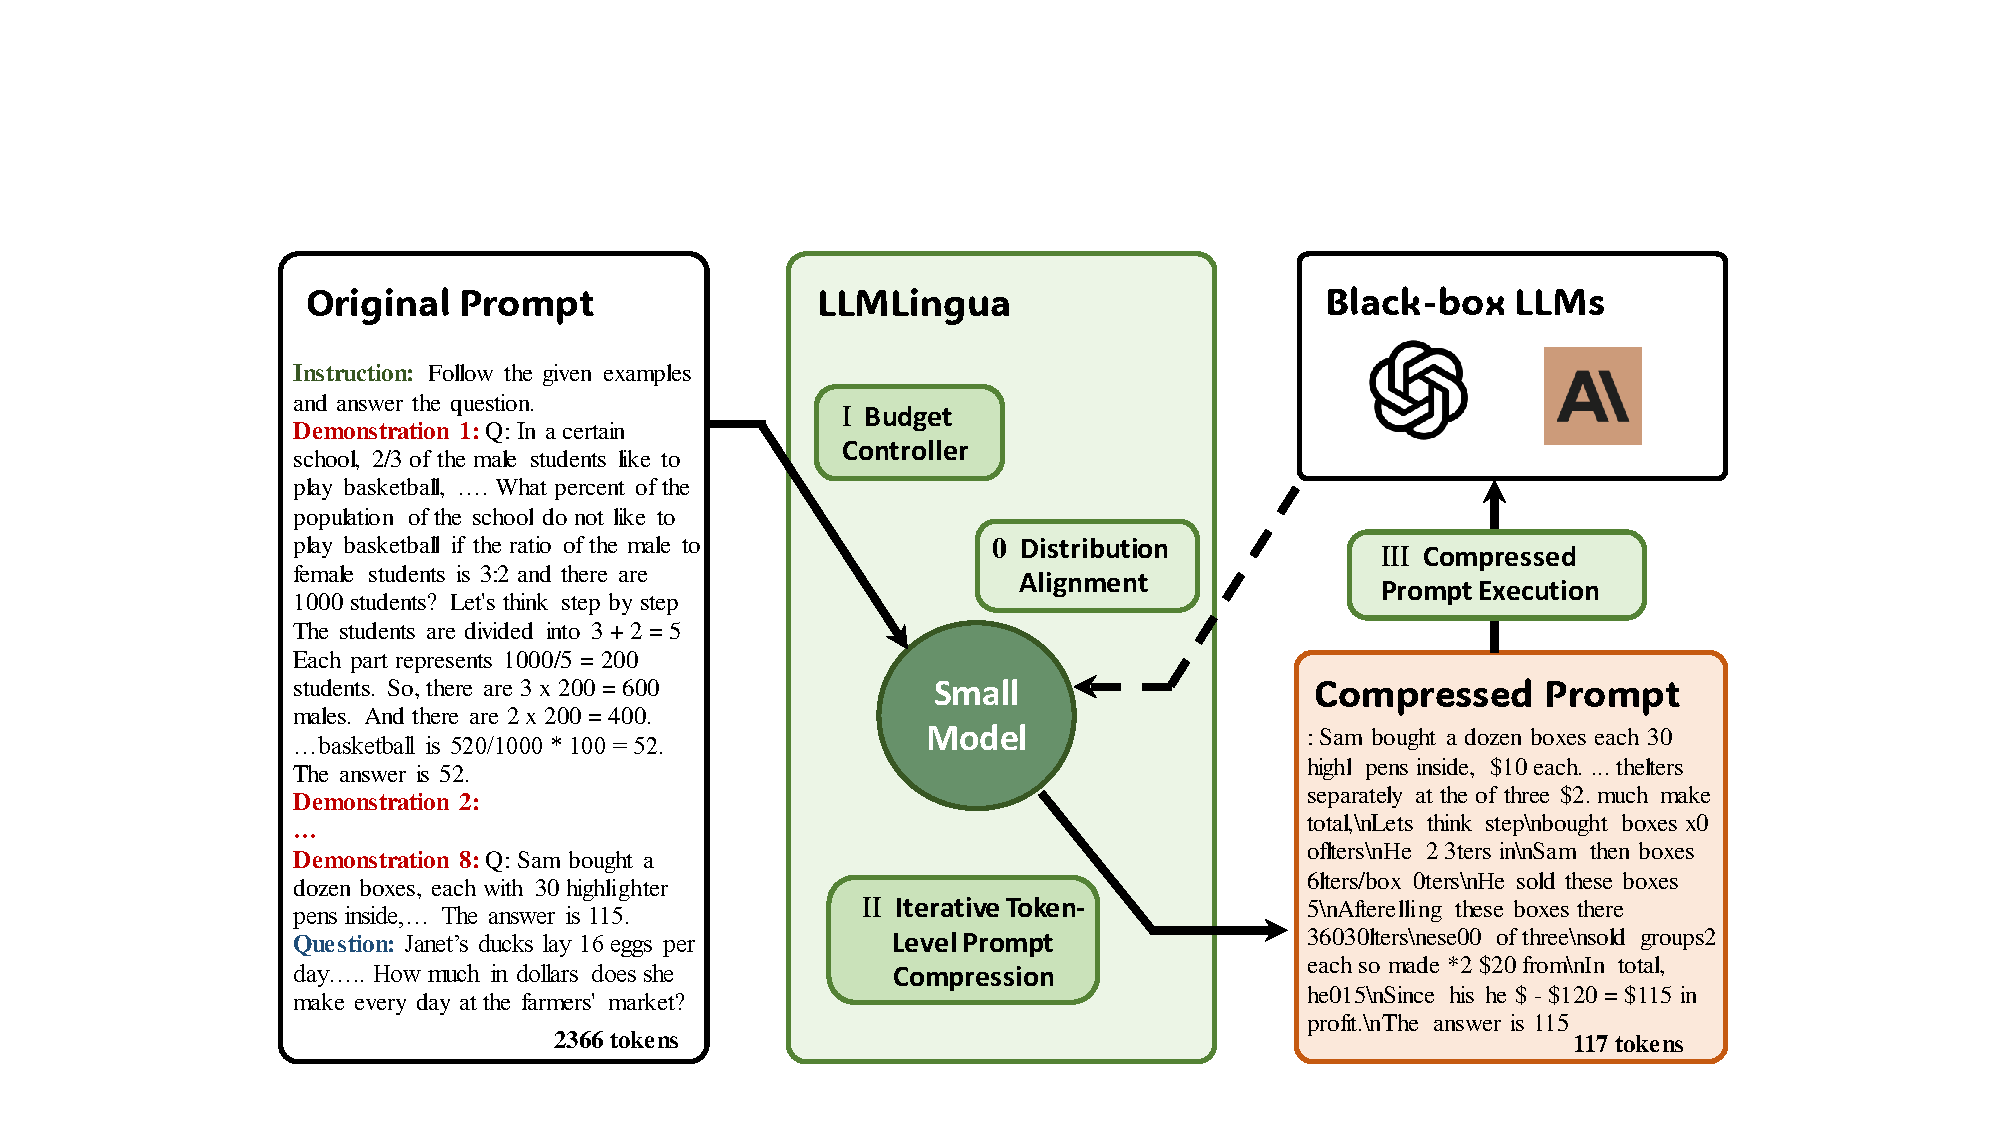
\includegraphics[width=0.98\linewidth]{figures/framework_LLMlingua.pdf}
    \caption{Framework of the proposed approach \textit{\sysname{}}.}
    \label{fig:framework}
\end{figure*}

% \subsection{Demonstration Selection}
% Furthermore, \citet{zhou2023efficient} introduces a reinforcement learning (RL) based algorithm that allocates a specific number of demonstrations for each question, thereby reducing prompt length.

\subsection{Out-of-Distribution (OoD) Detection}
Recently, a series of studies have been proposed for unsupervised OoD detection. % are also developed with computing perplexities.
% The distribution discrepancy between training and testing text can result in the suboptimal performance of pre-trained models on out-of-distribution data. 
% To a certain degree, prompt compression can also be regarded as a process for detecting relatively OoD tokens within a given text.
With only in-distribution texts available for learning, these methods either fine-tune a pre-trained language model \cite{arora2021types} or train a language model from scratch \cite{mai2022self}.
\citet{wu2023multi} analyze the characteristics of these methods and leverage multi-level knowledge distillation to integrate their strengths while mitigating their limitations.
Finally, perplexity output by the resulting language model is used as the indication of an example being OoD.

This paper also regards perplexity as a measurement of how well a language model predicts a sample.
In contrast to out-of-distribution detection, which identifies examples with high perplexities as indicative of unreliable predictions, we consider tokens with higher perplexity to be more influential during the inference process of language models. 
% Different from OoD detection where examples with high perplexities are bounded to unreliable predictions,
% we regard tokens with higher perplexity as those playing a more important role during LLMs' inference. 
% \textcolor{blue}{we ... perform prompt compression based on ppls:
% high ppls => rarely seen during training => more information => keep (otherwise drop).}


\subsection{LLMs as a Compressor}

Recently, many perspectives have interpreted large language models and unsupervised learning as a kind of compressor for world knowledge~\cite{ilya2023unsupervised, deletang2023language}, 
by using arithmetic coding~\cite{rissanen1976generalized,pasco1976source}. Our research can be viewed as an endeavor to further compress information within prompts by capitalizing on the compression-like characteristics of large language models.

